\question
{\center \bf COVID-19 Detector\\}
A hospital has reached out to us for help in classifying a large dataset of X-ray images to determine whether a person has COVID-19 or not. The hospital has been overwhelmed with patients and needs an automated system to assist their medical staff in diagnosing COVID-19 accurately and efficiently.


The project will consist of the following tasks:


\begin{itemize}
    \item
      \textbf{Task 1}: Read the gray images in the data set image by image, \href{https://ydjemmada.github.io/projects/xrays.zip}{Download the data set from here}.
    \item
      \textbf{Task 2}: Calculate the average of pixels having a value $\geq 128$ (near to white color) for each image
    \item
      \textbf{Task 3}: Classify the image based on the calculated average
      value:
    
      \begin{itemize}

      \item
        if the average $\leq 50$, the person is negative for Covid
      \item
        if the average $>50$ and $\leq 60$, the person is
        suspected to have Covid
      \item
        if the average $>60$, the person has Covid
      \end{itemize}
    \item
      \textbf{Task 4}: Process the images depending on their Covid status:
    
      \begin{itemize}

      \item
        Convert the gray images to RGB format
      \item
        For negative Covid images, add a green border to the image
      \item
        For suspected Covid images, add an orange border to the image
      \item
        For confirmed Covid images:
    
        \begin{itemize}

        \item
          Split the image vertically into two parts
        \item
          Calculate the average pixel value near to white for each part
        \item
          Determine which part of the image has a higher average value
        \item
          Add a red border to the original image on the side of the sick
          lung
        \end{itemize}
      \end{itemize}
    \item
      \textbf{Task 5}: Save the final result image to a folder named \verb|results|
    \end{itemize}
\begin{center}
        \begin{minipage}{.27\linewidth}
            \begin{figure}[H]
                \centering
                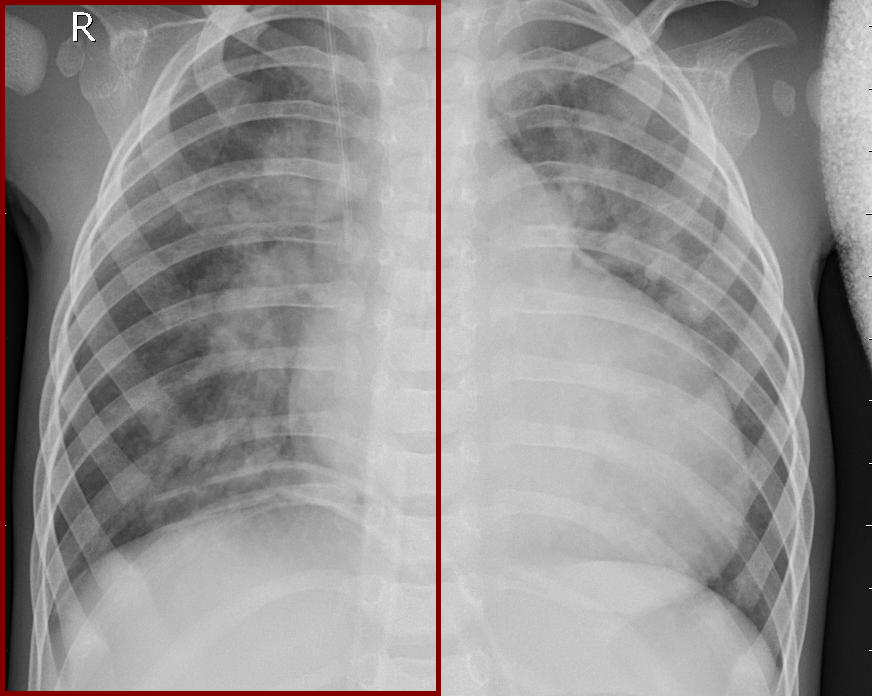
\includegraphics[width=110px]{red_border.png}
            \end{figure}
        \end{minipage}
        \begin{minipage}{.27\linewidth}
            \begin{figure}[H]
                \centering
                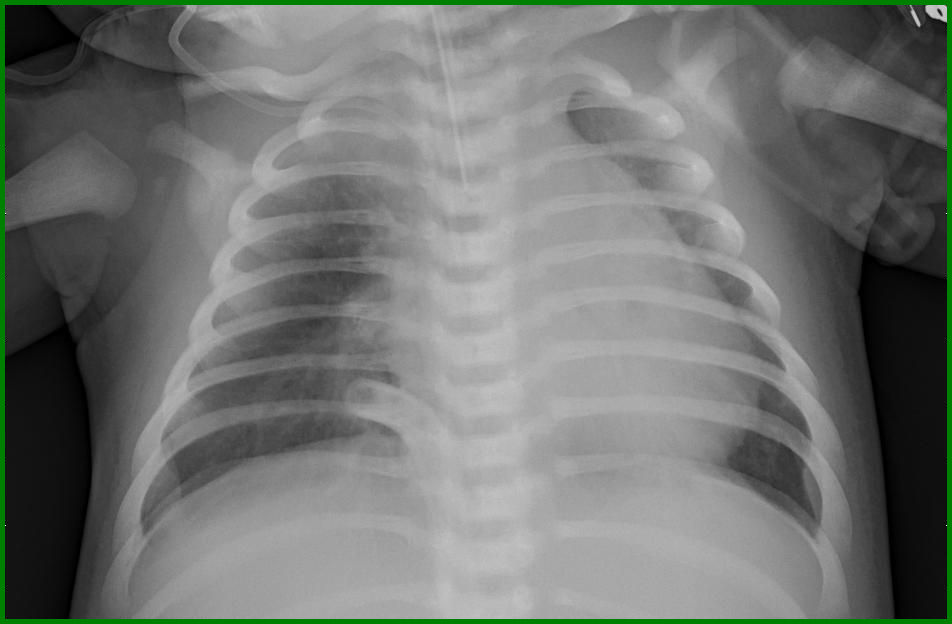
\includegraphics[width=110px]{green_border.png}
            \end{figure}
        \end{minipage}
        \begin{minipage}{.27\linewidth}
            \begin{figure}[H]
            \centering
                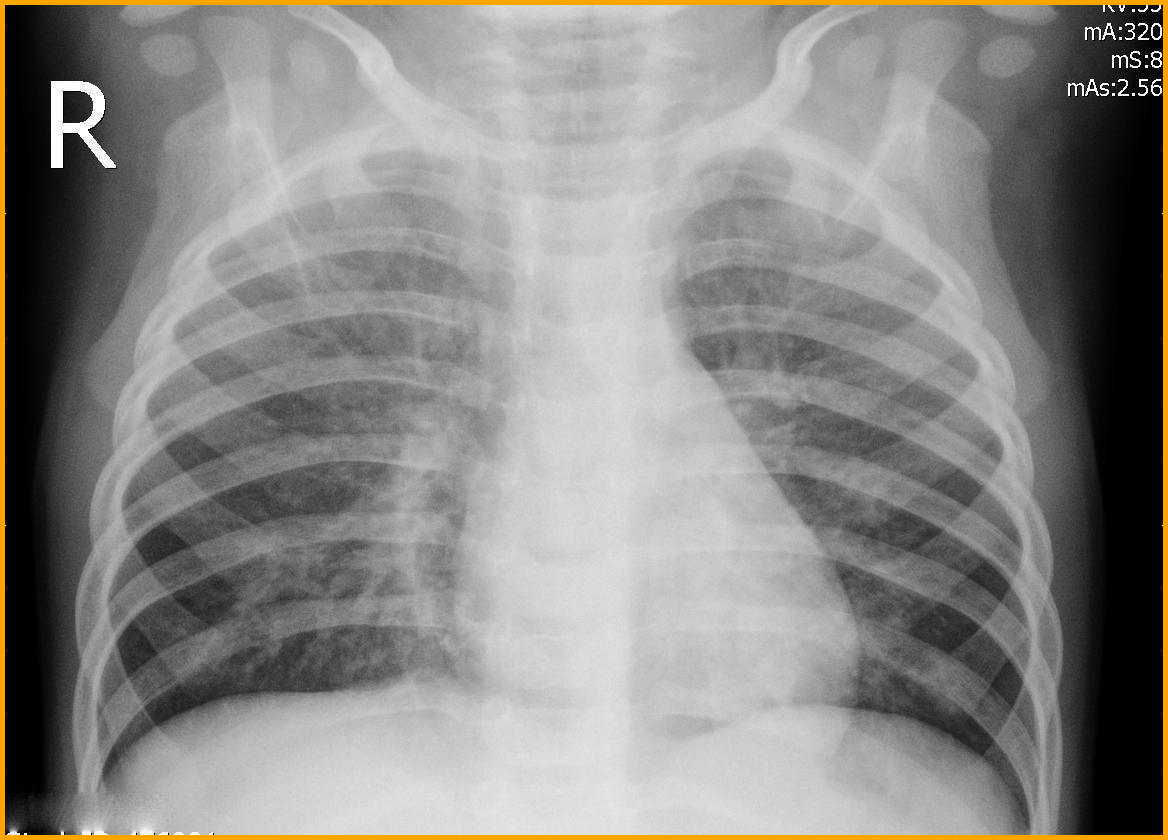
\includegraphics[width=110px]{orange_border.png}
            \end{figure}
        \end{minipage}
\end{center}

                  
    
    You can further break down each task into subtasks and write code to
    accomplish each subtask.
\newpage